\documentclass{book}
\usepackage{commeunjeustyle}
\begin{document}


\chapter*{Espaces préhilbertiens réels}

En algèbre linéaire, un espace préhilbertien réel est un espace vectoriel réel avec une structure supplémentaire appelée produit scalaire. Cette structure supplémentaire associe chaque couple de vecteurs à une quantité scalaire connue sous le nom de produit scalaire des vecteurs. Le produit scalaire permet l'introduction rigoureuse de notions géométriques intuitives telles que la longueur d'un vecteur ou l'angle entre deux vecteurs. Il permet de définir la notion d'orthogonalité entre vecteurs (produit scalaire nul). Les espaces préhilbertiens réels généralisent les espaces euclidiens aux espaces vectoriels de toute dimension (éventuellement infinie), et sont étudiés en analyse fonctionnelle.\\
Un produit scalaire induit naturellement une norme associée  donc un espace préhilbertien réel est également un espace vectoriel normé.

\section{Produit scalaire et norme}
\subsection{Produit scalaire}
\begin{Definition}[Produit scalaire]
Soit $E$ un $\R$-espace vectoriel de dimension finie ou infinie.
Un \defi{produit scalaire} sur $E$ est une forme bilinéaire symétrique définie positive sur $E$.
Autrement dit, un \defi{produit scalaire} sur $E$ est une application $\varphi:E^2\to \R$
\begin{itemize}
\item \defi{bilinéaire} :
  $\forall \vect{x},\vect{y},\vect{z}\in E, \forall \lambda ,\mu \in \R$
  $$ \varphi (\lambda \vect{x}+\mu \vect{y},\vect{z}) = \lambda \varphi (\vect{x},\vect{z}) + \mu \varphi (\vect{y},\vect{z})\text{ par rapport à la première variable}, $$
  $$ \varphi (\vect{x},\lambda \vect{y}+\mu \vect{z}) = \lambda \varphi (\vect{x},\vect{y}) + \mu \varphi (\vect{x},\vect{z})\text{ par rapport à la seconde variable}. $$
\item \defi{symétrique} : $\forall \vect{x},\vect{y}\in E, \quad  \varphi (\vect{y},\vect{x}) = \varphi (\vect{x},\vect{y}).$
\item \defi{définie} : $\forall \vect{x}\in E, \quad \varphi (\vect{x},\vect{x})=0 \Longrightarrow \vect{x} = \vect{0}_E$,
\item \defi{positive} : $\forall \vect{x}\in E,\quad \varphi (\vect{x},\vect{x})\geq 0.$ 
\end{itemize}
\end{Definition}
Il suffit de vérifier la linéarité à gauche et la symétrie pour justifier la bilinéarité.
\begin{Remarque}
A ce stade, les notions de norme et d'angle ne sont pas définies. Le produit scalaire est définie indépendamment d'une relation du type   $\langle \vect{x}, \vect{y} \rangle = \|\vect{x}\|\|\vect{y}\| \cos(\vect{x}, \vect{y})$. En réalité, dans la théorie des espaces préhilbertiens réels, la définition du produit scalaire est première et les notion de norme et d'angle viennent après.\\
Norme : $\|\vect{x}\|=\sqrt{\langle \vect{x}, \vect{x} \rangle}$.\\
Angle : $\theta=\arccos{\frac{\langle \vect{x}, \vect{y} \rangle}{\|\vect{x}\|\|\vect{y}\| }}$
\begin{center}
        \begin{tikzpicture}[very thick]
          \draw[-latex] (0,0) -- (3,0)  node[above]{$\vect{x}$};
          \draw[-latex] (0,0) -- (1, 3)  node[ right]{$\vect{y}$};
			\draw (3,0) coordinate (a) -- (0,0) coordinate (b) -- (1,3) coordinate (c)  pic["$\theta=\arccos{\frac{\langle \vect{x}, \vect{y} \rangle}{\|\vect{x}\|\|\vect{y}\| }}$", draw=orange, <->, angle eccentricity=1.2, angle radius=2cm]
    {angle=a--b--c};
        \end{tikzpicture}
\end{center}
\end{Remarque} 
\begin{Definition}[Espace préhilbertien réel]
Un \defi{espace préhilbertien réel}  est un $\R $-espace vectoriel $E$ muni d'un produit scalaire.\\
On note le produit scalaire généralement $\langle \vect{x}, \vect{y} \rangle$, $\langle \vect{x} \mid \vect{y} \rangle$, $(\vect{x},\vect{y})$, $(\vect{x}\mid \vect{y})$ ou encore $\vect{x}.\vect{y}$.\\
Un espace préhilbertien réel de dimension finie est appelé \defi{espace euclidien}.
\end{Definition}
\begin{DefinitionProposition}[Produit scalaire canonique sur $\R^n$]
Le \defi{produit scalaire canonique} est défini par  
$$\forall \vect{x} = ( x_1, \dots, x_n),\vect{y} =( y_1, \dots, y_n) \in\R^n :\quad \PS{\vect{x}}{\vect{y}} =\sum_{i=1}^n x_i \, y_i.  $$
Si on pose $X=\begin{pmatrix}
x_1\\ \vdots \\ x_n 
\end{pmatrix}$ et $Y=\begin{pmatrix}
y_1\\ \vdots \\ y_n 
\end{pmatrix}$, on a $\PS{\vect{x}}{\vect{y}}=\transposee{X}Y.$
\end{DefinitionProposition}
Ainsi défini, nous retrouvons le produit scalaire usuel défini dans le plan $\R^2$. Par exemple si $\vect{x} = ( x_1, x_2),\vect{y} =( y_1, y_2)$, on a  $\PS{\vect{x}}{\vect{y}} =x_1 y_1+x_2 y_2$.
\begin{Demonstration}
\begin{itemize}
\item \emph{symétrique} : $\PS{\vect{x}}{\vect{y}}=\transposee{X}Y  \overbrace{=}^{\text{matrice carré de taille 1}} \transposee{(\transposee{X}Y)} = \transposee{Y}X =\PS{\vect{y}}{\vect{x}}.$
\item \emph{bilinéaire} : par symétrie la linéarité par rapport à la seconde variable suffit,   $$\PS{\vect{x}}{\lambda \vect{y}_1+\mu \vect{y}_2}=\transposee{X}(\lambda Y_1+\mu Y_2)  =\lambda \transposee{X} Y_1+\mu \transposee{X} Y_2=\lambda \PS{\vect{x}}{\vect{y}_1}+\mu \PS{\vect{x}}{\vect{y}_2}  .$$
\item \emph{positive}: $\PS{\vect{x}}{\vect{x}}=\sum_{i=1}^n x_i^2 \geq 0.$
\item \emph{définie}: $\PS{\vect{x}}{\vect{x}}=\sum_{i=1}^n \overbrace{x_i^2}^{\geq 0} = 0$, alors  $x_i=0$ pour tout i, soit $\vect{x}=\vect{0}_{\R^n}$.
\end{itemize}
\end{Demonstration}
\begin{Exemple}[Non unicité du produit scalaire]
L'application $(X,Y)\to\transposee{X}\begin{pmatrix}
2&1 \\1&2
\end{pmatrix}Y$  est un produit scalaire sur $\R^2$ distinct du produit scalaire canonique.
\begin{itemize}
\item \emph{symétrique} : $\transposee{X}\begin{pmatrix}
2&1 \\1&2
\end{pmatrix}Y  \overbrace{=}^{\text{matrice carré de taille 1}} \transposee{(\transposee{X}\begin{pmatrix}
2&1 \\1&2
\end{pmatrix}Y)} =\transposee{Y}\transposee{\begin{pmatrix}
2&1 \\1&2
\end{pmatrix}}X = \transposee{Y}\begin{pmatrix}
2&1 \\1&2
\end{pmatrix}X .$
\item \emph{bilinéaire} : par symétrie la linéarité par rapport à la seconde variable suffit,   $$\transposee{X}\begin{pmatrix}
2&1 \\1&2
\end{pmatrix}(\lambda Y_1+\mu Y_2)  =\lambda \transposee{X}\begin{pmatrix}
2&1 \\1&2
\end{pmatrix} Y_1+\mu \transposee{X}\begin{pmatrix}
2&1 \\1&2
\end{pmatrix} Y_2.$$
\item \emph{positive}: $\transposee{X}\begin{pmatrix}
2&1 \\1&2
\end{pmatrix}X=2x_1^2+2x_1x_2+2x_2^2=x_1^2+x_2^2 +(x_1+x_2)^2\geq 0 .$
\item \emph{définie}: $\transposee{X}\begin{pmatrix}
2&1 \\1&2
\end{pmatrix}X= x_1^2+x_2^2 +(x_1+x_2)^2 = 0$, alors  $x_1=x_2=0$ , soit $X=\begin{pmatrix}
0 \\0
\end{pmatrix}$.
\end{itemize}
\end{Exemple}
\begin{Exemple}[Sur les fonctions continues]
L'application $(f,g)\to \int_0^1 f(t)g(t)\,\mathrm{dt} $ est un produit scalaire sur  $\mathcal{C}([0,1],\R )$.\\
Symétrie, bilinéaire et positivité évidentes.\\Pour définie, 
$\PS{f}{f}=\int_0^1 f^2(t)\,\mathrm{dt}=0$ implique que $f^2(t)=0$ pour tout $t\in[0,1]$ car $f^2$ est une fonction continue et positive. Donc $f=0$.
\end{Exemple}
\begin{Exemple}[Sur les polynômes]
L'application $(P,Q)\to \sum_{k=0}^n  P(k)Q(k) $ est un produit scalaire sur  $\R_n[X]$.\\
Symétrie, bilinéaire et positivité évidentes.\\Pour définie, 
$\PS{P}{P}=\sum_{k=0}^n  P^2(k)$ implique que $P$ admet $n+1$ racines donc $P=0$ car $\deg P \leq n$.
\end{Exemple}
\begin{Exemple}[Sur les matrices carrés]
L'application $(A,B)\to \Tr (\transposee{A}B)$ est un produit scalaire sur  $\Mn{\R}$.
\begin{itemize}
\item \emph{symétrique} : $\PS{A}{B} =\Tr (\transposee{A}B)  \overbrace{=}^{\Tr (\transposee{M})=\Tr (M) }\Tr (\transposee{(\transposee{A}B)})= \Tr (\transposee{B}A) =\PS{B}{A}$
\item \emph{bilinéaire} : par symétrie la linéarité par rapport à la seconde variable suffit,   $$\PS{A}{\lambda B_1+\mu  B_2 }= \Tr (\transposee{A}(\lambda B_1+\mu  B_2))=\lambda\Tr (\transposee{A}B_1)+\mu\Tr (\transposee{A}B_2)= \lambda\PS{A}{ B_1} +\mu  \PS{A}{B_2 }.$$
\item \emph{positive}: Rappels : coefficient d'un produit de matrice $(AB)_{i j}=\sum_{k=1}^n a_{i k}b_{k j}$ et trace $\Tr (C)=\sum_{k=1}^{n}c_{kk}$.\\
On a $$\PS{A}{A}=\Tr (\transposee{A}A) = \sum_{j=1}^{n}  (\transposee{A} A)_{j j} =\sum_{j=1}^{n} \sum_{i=1}^{n}a_{i j} a_{i j}=\sum_{j=1}^{n} \sum_{i=1}^{n} a^2_{i j}\geq 0$$
\item \emph{définie}: $\sum_{j=1}^{n} \sum_{i=1}^{n} a^2_{i j}=0$ implique que  $a_{i j}=0$ pour tout $i,j\in \Intf{1}{n}$, donc $A=0$.
\end{itemize}
\end{Exemple}
\subsection{Norme associée à une produit scalaire}
\begin{Definition}
Soit $(E,\PS{.}{.})$ un espace préhilbertien réel.\\
On appelle \defi{norme associée} l'application $\norme{.}: E\to \R $ définie par 
$$ \forall \vect{x}\in E:\quad  \norme{\vect{x}} =\sqrt{\PS{\vect{x}}{\vect{x}}}.$$
On appelle \defi{distance} de $\vect{x}$ à $\vect{y}$ le réel positif $d(\vect{x},\vect{y}) =\norme{\vect{x}-\vect{y}} $.\\ 
Le vecteur $\vect{x}$ est dit \defi{unitaire} si $\norme{\vect{x}}=1.$
\end{Definition}
\begin{Remarque}
Si $\vect{x}\neq \vect{0}$, le vecteur $\frac{\vect{x}}{\norme{\vect{x}}}$ est unitaire.
\end{Remarque}
\begin{Proposition}[Identités remarquables de la norme associée]
Soit $(E,\PS{.}{.})$ un espace préhilbertien réel et $\vect{x},\vect{y}\in E$.
On a
\begin{itemize}
\item $\norme{\vect{x}+\vect{y}}^2 = \norme{\vect{x}}^2 + \norme{\vect{y}}^2 + 2\PS{\vect{x}}{\vect{y}}$
\item $\norme{\vect{x}-\vect{y}}^2 = \norme{\vect{x}}^2 + \norme{\vect{y}}^2 - 2\PS{\vect{x}}{\vect{y}}$
\item \propri{identité du parallélogramme}:
  $\norme{\vect{x}+\vect{y}}^2 + \norme{\vect{x}-\vect{y}}^2 = 2\bigl( \norme{\vect{x}}^2 + \norme{\vect{y}}^2 \bigr)$
\item \propri{identité de polarisation}:
  $\PS{\vect{x}}{\vect{y}} = \frac14 \bigl( \norme{\vect{x}+\vect{y}}^2 - \norme{\vect{x}-\vect{y}}^2 \bigr)$.
\end{itemize}
L'identité du parallélogramme signifie que, dans un parallélogramme, la somme des carrés des longueurs des diagonales est égale au double de la somme des carrés des longueurs des côtés.
\begin{center}
        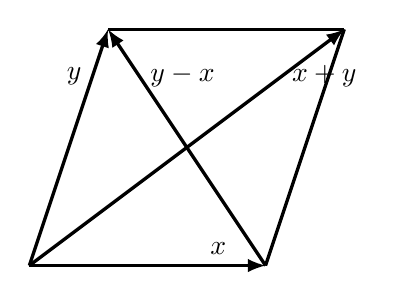
\begin{tikzpicture}[very thick]
          \draw[-latex] (0,0) -- (3,0)  node[pos=0.8,,above]{$\vect{x}$};
          \draw[-latex] (0,0) -- (1, 3)  node[pos=0.8, left]{$\vect{y}$};
          \draw[-latex] (0,0) -- (4, 3)  node[pos=0.8, right]{$\vect{x}+\vect{y}$};
          \draw[-latex] (3,0) -- (1, 3)  node[pos=0.8, right]{$\vect{y}-\vect{x}$};
			\draw[-] (1,3) -- (4, 3)  ;
			\draw[-] (3,0) -- (4, 3)  ;
        \end{tikzpicture}
\end{center}
\end{Proposition}
\begin{Demonstration}
Pour la première identité, on a :
$$\norme{\vect{x}+\vect{y}}^2 = \PS{\vect{x}+\vect{y}}{\vect{x}+\vect{y}}\overbrace{=}^{\text{distributivité}}\PS{\vect{x}}{\vect{x}}+\PS{\vect{x}}{\vect{y}}+\PS{\vect{y}}{\vect{x}}+\PS{\vect{y}}{\vect{y}}\overbrace{=}^{\text{symétrie}}\norme{\vect{x}}^2 + \norme{\vect{y}}^2 + 2\PS{\vect{x}}{\vec{y}}.$$
La démonstration de la suivante est similaire. Les deux dernières identités sont des combinaisons des deux premières (+ et -). 
\end{Demonstration}

\begin{Theoreme}[Inégalité de Cauchy-Schwarz]
Soit $(E,\PS{.}{.})$ un espace préhilbertien réel.\\
Alors pour tout $\vect{x},\vect{y}\in E$, on a :
\[ | \PS{\vect{x}}{\vect{y}} | \leq  \norme{\vect{x}}\cdot \norme{\vect{y}}. \]
De plus, on a égalité si et seulement si $\vect{x}$ et $\vect{y}$ sont liés.
\end{Theoreme}
\begin{Demonstration}
Voir \url{https://www.youtube.com/watch?v=0AVLW1bTpLw}.\\
Dans $\R^2$, la démonstration est directe car $\PS{\vect{x}}{\vect{y}}=\norme{\vect{x}}\cdot \norme{\vect{y}}\cos(\theta)$  et $|\cos(\theta)|\leq 1$.
\begin{center}
        \begin{tikzpicture}[very thick]
          \draw[-latex] (0,0) -- (3,0)  node[above]{$\vect{x}$};
          \draw[-latex] (0,0) -- (1, 3)  node[ right]{$\vect{y}$};
			\draw (3,0) coordinate (a) -- (0,0) coordinate (b) -- (1,3) coordinate (c)  pic["$\theta$", draw=orange, <->, angle eccentricity=1.2, angle radius=2cm]
    {angle=a--b--c};
        \end{tikzpicture}
\end{center}
Dans le cas générale, lorsque $\vect{y} =  \vect{0}$, l'énoncé est clairement vrai, par conséquent on supposera $\vect{y}$ non nul.
\begin{itemize}
\item \textit{Inégalité} Posons, pour tout réel $t$, $P(t)=\norme{\vect{x}+t\vect{y}}^{2}$. Par construction, la fonction $P$ est  positive ou nulle. On a :
$$P(t)= \PS{\vect{x}+t\vect{y}}{\vect{x}+t\vect{y}}\overbrace{=}^{\text{bilinéarité}} \norme{\vect{x}}^2 +2t\PS{\vect{x}}{\vect{y}} +t^2  \norme{\vect{y}}^2$$
Comme $\vect{y}$ est non nul, $\norme{\vect{y}}^2$ est non nul également.  $P$ est donc une fonction polynomiale du second degré. $P$ étant positive ou nulle, son discriminant est négatif ou nul  :
$$4\PS{ \vect{x}}{\vect{y}}^{2}-4\norme{\vect{x}}^{2}\norme{\vect{y}}^{2}\leq 0 $$
Comme $t\to\sqrt{t}$ est croissante, on obtient l'inégalité de Cauchy-Schwarz
\[ | \PS{\vect{x}}{\vect{y}} | \leq  \norme{\vect{x}}\cdot \norme{\vect{y}}. \]
\item \textit{Égalité} Si $(\vect{x}, \vect{y})$ est une famille liée alors, il existe $\lambda\in\ R$ tel que $\vect{x} = \lambda\vect{y}$. On a:
$$|\PS{\vect{x}}{\vect{y}}|=|\PS{\lambda\vect{y}}{\vect{y}}|=|\lambda| \norme{\vect{y}}^{2}=\norme{\vect{x}}\norme{\vect{y}}.$$
Réciproquement, si $|\PS{\vect{x}}{\vect{y}}| = \norme{\vect{x}}\norme{\vect{y}}$ alors le discriminant ci-dessus est nul donc $P$ admet une racine réelle (double) $t$, et pour ce $t$ on a
$$ \norme{\vect{x}+t\vect{y}}^{2}=0\overbrace{\Longrightarrow}^{\text{définie}} \vect{x}+t\vect{y} =\vect{0}.$$
Donc $(\vect{x}, \vect{y})$ est une famille liée.
\end{itemize} 
\end{Demonstration}
\begin{Exemple}
Pour tout $x_1,\dots,x_n\in \R:\quad \left(\sum_{i=1}^n x_i\right)^2\leq n \sum_{i=1}^n x_i^2$ avec égalité si et seulement si $x_1=\dots=x_n$.\\
Il suffit d'appliquer l'inégalité de Cauchy-Schwarz  aux vecteurs $(x_1,\dots,x_n)$ et $(1,\dots,1)$ de $ \R^n$ muni du produit scalaire canonique.   
\end{Exemple}
\begin{Exemple}
Pour tout $f\in \mathcal{C}([0,1],\R ):\quad |\int_0^1f(t)\,\mathrm{dt}|\leq \sqrt{\int_0^1f^2(t)\,\mathrm{dt}}   $.\\
Il suffit d'appliquer l'inégalité de Cauchy-Schwarz  aux vecteurs $f$ et $x\to 1$ de $ \mathcal{C}([0,1],\R ) $ muni du produit scalaire   $\PS{f}{g}= \int_0^1 f(t)g(t)\,\mathrm{dt}.$
\end{Exemple}




\begin{Corollaire}[Norme sur $E$]
Soit $(E,\PS{.}{.})$ un espace préhilbertien réel.\\
Alors la norme associée $\norme{.}$ est une \propri{norme} sur $E$, c'est-à-dire vérifie ces propriétés :
\begin{itemize}
\item \propri{Homogène :} $\norme{\lambda \vect{x}}=|\lambda|\norme{\vect{x}}.$ 
\item \propri{Définie :} $\norme{\vect{x}}=0\Longrightarrow \vect{x} =0.$
\item \propri{Inégalité triangulaire :}  $\norme{\vect{x}+\vect{y}}\leq \norme{\vect{x}}+\norme{\vect{y}}.$
\end{itemize}
\end{Corollaire}
Cette norme fournit une structure d'espace vectoriel normé sur $E$. On peut donc parler de convergence sur $E$, de topologie sur $E$, etc.
\begin{Demonstration}
\begin{itemize}
\item \textit{Homogène :} $\norme{\lambda \vect{x}}=\sqrt{\PS{\lambda \vect{x}}{\lambda \vect{x}}}=|\lambda|\sqrt{\PS{ \vect{x}}{\vect{x}}}=|\lambda|\norme{\vect{x}}.$ 
\item \textit{Définie :} $\norme{\vect{x}}=\sqrt{\PS{ \vect{x}}{\vect{x}}}=0\Longrightarrow \PS{ \vect{x}}{\vect{x}} =0\Longrightarrow \vect{x} =0$
\item \textit{Inégalité triangulaire :} $$\norme{\vect{x}+\vect{y}}^2=\norme{\vect{x}}^2+2\PS{\vect{x}}{\vect{y}}+  \norme{\vect{y}}^2\overbrace{\leq}^{\text{Inégalité de Cauchy-Schwarz}}\norme{\vect{x}}^2+2\norme{\vect{x}} \norme{\vect{y}} + \norme{\vect{y}}^2 =(\norme{\vect{x}}+\norme{\vect{y}})^2.$$
Comme $t\to\sqrt{t}$ est croissante, on obtient l'inégalité : $\norme{\vect{x}+\vect{y}}\leq \norme{\vect{x}}+\norme{\vect{y}}.$
\end{itemize}
\end{Demonstration}
\section{Orthogonalité}
On considère un un espace préhilbertien réel $(E,\PS{.}{.})$.

%
%% -----------------------------------------------------------------------------
\subsection{Vecteurs orthogonaux}

\begin{Definition}[Vecteurs orthogonaux]
Soit $\vect{x},\vect{y}\in E$.\\
On dit que les vecteurs $\vect{x}$ et $\vect{y}$ sont \defi{orthogonaux} si $\PS{\vect{x}}{\vect{y}} = 0$.\\
On note $\vect{x} \perp \vect{y}$.
\end{Definition}
En géométrie d'Euclide, la notion d'orthogonalité est associée  à l'angle droit et est première par rapport au produit scalaire. Dans cette théorie générale, elle est seconde et est relative au produit scalaire. En particulier, en fonction du choix du produit scalaire, deux vecteurs peuvent être orthogonaux ou non.
\begin{Exemple}
Les vecteurs $(1,0)$ et $(0,1)$ sont orthogonaux par rapport au produit scalaire canonique $\transposee{X}Y$  mais ne le sont pas rapport au produit scalaire $\transposee{X}\begin{pmatrix}
2&1 \\1&2
\end{pmatrix}Y$ car $\begin{pmatrix}
1 &0
\end{pmatrix}\begin{pmatrix}
2&1 \\1&2
\end{pmatrix}\begin{pmatrix}
0 \\1
\end{pmatrix}=1$.
\end{Exemple}
\begin{Exemple}
$E=\mathcal{C}([0,2\pi],\R )$ et $\PS{f}{g}= \int_0^{2\pi} f(t)g(t)\,\mathrm{dt} $.\\
Comme $\PS{\cos}{\sin}=0$, les vecteurs $\cos$ et $\sin$ sont orthogonaux. 
\end{Exemple}   
\begin{Theoreme}[Pythagore]
Soit $\vect{x},\vect{y}\in E$.\\
$$\norme{\vect{x}+\vect{y}}^2=\norme{\vect{x}}^2+\norme{\vect{y}}^2 \Leftrightarrow \PS{\vect{x}}{\vect{y}} = 0.$$
\newcommand{\pythagwidth}{3cm}
\newcommand{\pythagheight}{2cm}

\begin{center}
\begin{tikzpicture}
  \coordinate [label={below right:$A$}] (A) at (0, 0);
  \coordinate [label={above right:$B$}] (B) at (0, \pythagheight);
  \coordinate [label={below left:$C$}] (C) at (-\pythagwidth, 0);
  \coordinate (D1) at (-\pythagheight, \pythagheight + \pythagwidth);
  \coordinate (D2) at (-\pythagheight - \pythagwidth, \pythagwidth);
  \coordinate  (A1) at (-\pythagwidth*3/4 , \pythagheight*3/2);
  \coordinate  (B1) at (\pythagheight/2, \pythagheight/2);
  \coordinate  (C1) at (-\pythagwidth/2, -\pythagwidth/2);
  \coordinate  (E1) at (\pythagheight*3/2, \pythagwidth);
  \coordinate  (E2) at (\pythagheight*2/2, \pythagwidth);
  \draw [very thick] (A) -- (C) -- (B) -- (A);
  \newcommand{\ranglesize}{0.3cm}
  \draw (A) -- ++ (0, \ranglesize) -- ++ (-\ranglesize, 0) -- ++ (0, -\ranglesize);
  \draw [dashed] (A) -- node [below] {$b$} ++ (-\pythagwidth, 0)
            -- node [right] {} ++ (0, -\pythagwidth)
            -- node [above] {} ++ (\pythagwidth, 0)
            -- node [left] {} ++ (0, \pythagwidth);
  \draw (B1) node{$c^2$};
  \draw (C1) node{$b^2$};	 	  
  \draw [dashed] (A) -- node [right] {$c$} ++ (0, \pythagheight)
            -- node [below] {} ++ (\pythagheight, 0)
            -- node [left] {} ++ (0, -\pythagheight)
            -- node [above] {} ++ (-\pythagheight, 0);
  \draw [dashed] (C) -- node [above left] {$a$} (B)
                     -- node [below left] {} (D1)
                     -- node [below right] {} (D2)
                     -- node [above right] {} (C);
  \draw (B1) node{$c^2$};
  \draw (C1) node{$b^2$};
  \draw (A1) node{$a^2$};
  \draw (E1) node{$a^2=b^2+c^2$};			                    
\end{tikzpicture}\\
Illustration du théorème de Pythagore dans le plan
\end{center}
\end{Theoreme}
\begin{Demonstration}
$\norme{\vect{x}+\vect{y}}^2=\norme{\vect{x}}^2+\norme{\vect{y}}^2+2\PS{\vect{x}}{\vect{y}}$, donc  $\norme{\vect{x}+\vect{y}}^2=\norme{\vect{x}}^2+\norme{\vect{y}}^2 \Leftrightarrow \PS{\vect{x}}{\vect{y}} = 0.$
\end{Demonstration}
\begin{Proposition}
Le vecteur nul est le seul vecteur orthogonal à tout les autres.
\end{Proposition}
\begin{Demonstration}
Analyse : Soit $\vect{x}$ un vecteur orthogonal à tout les autres. En particulier, il est orthogonal à lui-même donc $\PS{\vect{x}}{\vect{x}}=0$, donc  $\vect{x}=\vect{0}$.\\
Synthèse : on vérifie que le vecteur nul est orthogonal à tout les autres.
\end{Demonstration}
\subsection{Famille orthogonales et orthonormales}   
\begin{Definition}
Soit $\mathcal{F} = (\vect{x}_1,\dots,\vect{x}_n)$ une famille de vecteurs de $E$.\\
La famille $\mathcal{F}$ est \defi{orthogonale} si 
$$\forall i,j\in \Intf{1}{n}:\quad i\neq j \Rightarrow \PS{\vect{x}_i}{\vect{x}_j}=0.$$
La famille $\mathcal{F}$ est \defi{orthonormale}  si la famille est orthogonale et si les vecteurs sont unitaires ($\forall i\in \Intf{1}{n}:\norme{\vect{x}_i}=1$).\\
La famille $\mathcal{F}$ est une \defi{base orthonormale} si la famille une base et une famille orthonormale.
\end{Definition}
\begin{Theoreme}[Pythagore généralisée]
Soit $(\vect{x}_1,\dots,\vect{x}_n)$ une famille orthogonale de vecteurs de $E$.\\
Alors \[ \norme{\sum_{i=1}^n \vect{x}_i }^2 = \sum_{i=1}^n \norme{\vect{x}_i}^2. \]
\end{Theoreme}
\begin{Proposition}[libre]
Une famille orthogonale dont tous les vecteurs sont non nuls est libre.\\
En particulier, une famille orthonormale est libre.
\end{Proposition}
Si $E$ est de dimension finie, une famille orthonormale contient au plus $\dim E$ vecteurs. Si elle contient $\dim E$, c'est une base. 
\begin{Demonstration}
Soit $(\vect{x}_1,\dots,\vect{x}_n)$ une famille orthogonale dont tous les vecteurs sont non nuls.\\
Soit $\lambda_1,\dots,\lambda_n\in\R $ tel que $\lambda_1\vect{x}_1+\dots+\lambda_n\vect{x}_n=\vect{0}$.\\
Pour tout $j\in \Intf{1}{n}$, on a :
$$\PS{\vect{x}_j}{\sum_{i=1}^n\lambda_i\vect{x}_i}=\sum_{i=1}^n\lambda_i\PS{\vect{x}_j}{\vect{x}_i}\overbrace{=}^{\text{famille orthogonale}}\lambda_j \norme{\vect{x}_j}^2=0 $$ 
Comme $\norme{\vect{x}_j}\neq 0$, $\lambda_j=0$ pour tout $j\in \Intf{1}{n}$. Donc la famille est libre.
\end{Demonstration}
\begin{Proposition}[Coordonnées dans une base orthonormale]
Soit $E$ un espace euclidien de dimension $n$ et $(\vect{e}_1,\dots,\vect{e}_n)$ une base orthonormale de $E$.
Alors
$$\forall \vect{x}\in E :  \quad  \vect{x}=\PS{\vect{x}}{\vect{e}_1} \vect{e}_1+\dots+\PS{\vect{x}}{\vect{e}_n}\vect{e}_n=\sum_{i=0}^n\PS{\vect{x}}{\vect{e}_i}\vect{e}_i.$$ 
\end{Proposition}
\begin{Demonstration}
Soit $\vect{x}\in E$. Il existe $x_1,\dots,x_n\in\R$ tel que $\vect{x}= x_1 \vect{e}_1+\dots+x_n\vect{e}_n=\sum_{i=0}^n x_i\vect{e}_i.$\\
Pour tout $j\in \Intf{1}{n}$, on a :
$$\PS{\vect{x}}{\vect{e}_j} = \PS{\sum_{i=1}^nx_i\vect{e}_i}{\vect{e}_j}=\sum_{i=1}^nx_i\PS{\vect{e}_i}{\vect{e}_j}\overbrace{=}^{\text{famille orthonormale}}x_j.$$ 
\end{Demonstration} 
\begin{Proposition}[Expression du produit scalaire et de la norme dans une base orthonormale]
Soit $E$ un espace euclidien de dimension $n$ et $(\vect{e}_1,\dots,\vect{e}_n)$ une base orthonormale de $E$.
Soit $\vect{x}= \sum_{i=1}^n x_i \vect{e}_i,\vect{y}=\sum_{i=1}^n y_i \vect{e}_i\in E$.\\
Alors :
$$\PS{\vect{x}}{\vect{y}}=\sum_{i=1}^n x_iy_j=\sum_{i=1}^n \PS{\vect{x}}{\vect{e}_i}\PS{\vect{y}}{\vect{e}_i}=   \transposee {X}Y\quad \text{et}\quad \norme{\vect{x}}^2=\sum_{i=1}^n \PS{\vect{x}}{\vect{e}_i}^2 =\transposee {X}X$$
\end{Proposition} 
\begin{Demonstration}
$$\PS{\vect{x}}{\vect{y}} = \PS{\sum_{i=1}^n x_i \vect{e}_i }{\sum_{j=1}^n y_j \vect{e}_j}\overbrace{=}^{\text{bilinéarité}}\sum_{i=1}^n\sum_{j=1}^n x_i y_j\PS{  \vect{e}_i }{ \vect{e}_j}=\sum_{i=1}^n x_iy_j. $$
\end{Demonstration}
Ainsi, en dimension finie, tous les produits scalaires se ramènent au produit scalaire canonique via le choix d'une base orthonormale. Dans le cours sur les espaces vectoriels, on a prouvé l'existence d'une base. Le théorème prouve que l'on peut construire une base orthonormale à partir d'une base quelconque.  

\begin{Theoreme}[Algorithme d'orthonormalisation de Gram-Schmidt]
Soit $(\vect{x}_1,\dots,\vect{x}_p)$ une famille \emph{libre} de vecteurs de $E$.\\
Alors il existe une \propri{unique} famille $(\vect{e}_1,\dots,\vect{e}_p)$  de vecteurs de $E$
telle que
\begin{itemize}
\item la famille $(\vect{e}_1,\dots,\vect{e}_p)$ est orthonormale,
\item pour tout $n\in \Intf{1}{p}$, \[ \Vectt (\vect{x}_1,\dots,\vect{x}_n) = \Vectt (\vect{e}_1,\dots,\vect{e}_n), \]
\item pour tout $n\in \Intf{1}{p}$, $\PS{\vect{x}_n}{\vect{e}_n} > 0$.
\end{itemize}
De plus, on peut la construire avec les formules suivantes:
\begin{itemize}
\item $\vect{e}_1 = \frac{\vect{x}_1}{\norme{\vect{x}_1}}$;
\item pour $n\in \Intf{2}{p}$, on note
  \[ \vect{e'}_n = \vect{x}_n - \sum_{k=1}^{n-1} \PS{\vect{e}_k}{\vect{x}_n} \vect{e}_k; \]
	\[\vect{e}_n = \frac{\vect{e'}_n}{\norme{\vect{e'}_n}}.\]
\end{itemize}
\end{Theoreme}
\begin{Demonstration}
Si $n=2$, on applique cette algorithme :
\begin{enumerate}
\item \textit{Normaliser $\vect{x_1}$ : } $\vect{e_1}=\frac{\vect{x_1}}{\norme{\vect{x_1}}}$
\item \textit{Projeter $\vect{x_2}$ sur la droite vectorielle  $\R \vect{x_1}$ : }$\PS{\vect{x_2}}{\vect{e_1}}\vect{e_1}$
\item \textit{Retrancher à $\vect{x_2}$ la composante suivante $\vect{e_1}$  : } $\vect{e'_2}= \vect{x_2} - \PS{\vect{x_2}}{\vect{e_1}}\vect{e_1}$
\item \textit{Normaliser $\vect{e'_2}$ : } $\vect{e_2}=\frac{\vect{e'_2}}{\norme{\vect{e'_2}}} $
\end{enumerate}
\begin{center}
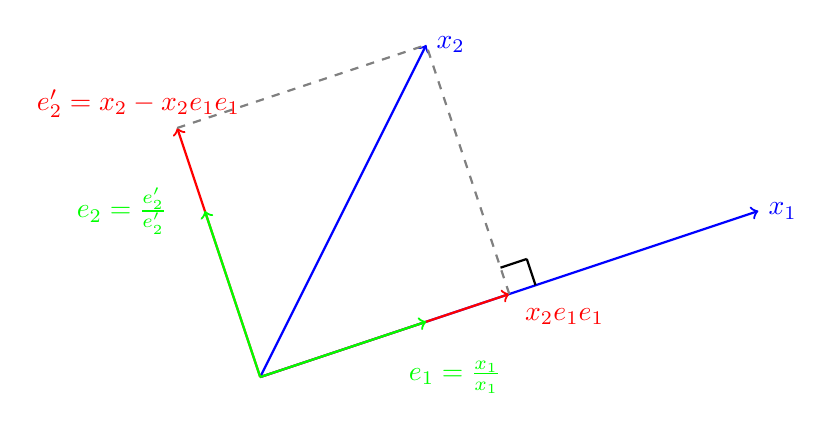
\begin{tikzpicture}[thick, scale=2]
%\draw[->,very thick] (0,0) -- +(100pt,0pt);
%\draw[->,very thick] (0,0) -- +(0pt,100pt);
\draw[->,blue] (0,0) -- +(90pt,30pt);
\draw[->,blue] (0,0) -- +(30pt,60pt);
\draw[->,red] (0,0) -- +(45pt,15pt);
\draw[->,red] (0,0) -- +(-15pt,45pt);
\draw[->,green] (0,0) -- +(30pt,10pt);
\draw[->,green] (0,0) -- +(-10pt,30pt);
\draw[dashed,gray] (45pt,15pt) -- (30pt,60pt);
\draw[dashed,gray] (-15pt,45pt) -- (30pt,60pt);
\draw (49.7434pt,16.5811pt) -- (48.1623pt,21.3246pt);
\draw (43.4189pt,19.7434pt) -- (48.1623pt,21.3246pt);
\draw (90pt,30pt) node[anchor=west] {${\color{blue} \vect{x_1}}$};
\draw (25pt,0pt) node[anchor=west] {${\color{green} \vect{e_1}=\frac{\vect{x_1}}{\norme{\vect{x_1}}} }$};
\draw (30pt,60pt) node[anchor=west] {${\color{blue} \vect{x_2}}$};
\draw (46pt,11pt) node[anchor=west] {${\color{red} \PS{\vect{x_2}}{\vect{e_1}}\vect{e_1}}$};
\draw (-22pt,45pt) node[anchor=south] {${\color{red}\vect{e'_2}=\vect{x_2} -\PS{\vect{x_2}}{\vect{e_1}}\vect{e_1} }$};
\draw (-35pt,30pt) node[anchor=west] {${\color{green} \vect{e_2}=\frac{\vect{e'_2}}{\norme{\vect{e'_2}}} }$};
\end{tikzpicture}
\end{center}
Plus généralement, le procédé de Gram-Schmidt construit $\vect{e_k}$ en retranchant à  $\vect{x_k}$ ses composantes selon $\vect{e_1},\dots, \vect{e_{k-1}}$ puis en le normalisant  :\\
\begin{tabular}{ll}
$\vect{e'_1}=\vect{x_1}$&$\vect{e_1}=\frac{\vect{e'_1}}{\norme{\vect{e'_1}}}$ \\
$\vect{e'_2}=\vect{x_2}-\PS{\vect{x_2}}{\vect{e_1}}\vect{e_1}$&$\vect{e_2}=\frac{\vect{e'_2}}{\norme{\vect{e'_2}}}$ \\
$\vect{e'_3}=\vect{x_2}-\PS{\vect{x_3}}{\vect{e_1}}\vect{e_1}-\PS{\vect{x_3}}{\vect{e_2}}\vect{e_2}$&$\vect{e_3}=\frac{\vect{e'_3}}{\norme{\vect{e'_3}}}$ \\
$\vdots$&$\vdots$ \\
$\vect{e'_k}=\vect{x_k}-\sum_{i=1}^{k-1}\PS{\vect{x_k}}{\vect{e_i}}\vect{e_i}$&$\vect{e_k}=\frac{\vect{e'_k}}{\norme{\vect{e'_k}}}$ \\
\end{tabular}\\
Démontrons par récurrence que $\vect{e'_k}$ est orthogonal à la famille $(\vect{e_1},\dots, \vect{e_{k-1})}$ pour $k\in \Intf{1}{n}$.\\
\begin{itemize}
\item \textit{Initialisation }: le vecteur  $\vect{e'_1}$ est orthogonal à la famille vide
\item \textit{Hérédité }: supposons la propriété vraie au rang $k$ et montrons qu'elle est vraie au rang $k+1$.\\
Soit $j\in\Intf{1}{k-1}$. On a :
$$\PS{\vect{e'_k}}{\vect{e_j}}=\PS{\vect{x_k}-\sum_{i=1}^{k-1}\PS{\vect{x_k}}{\vect{e_i}}\vect{e_i}}{\vect{e_j}}=\PS{\vect{x_k}}{\vect{e_j}}- \overbrace{\sum_{i=1}^{k-1}\PS{\vect{x_k}}{\vect{e_i}}\PS{ \vect{e_i}} {\vect{e_j}}}^{\text{ d'après HR } \PS{\vect{e_i}}{\vect{e_j}}=\delta_{i,j}} =\PS{\vect{x_k}}{\vect{e_j}}-\PS{\vect{x_k}}{\vect{e_j}}\PS{ \vect{e_j}} {\vect{e_j}}=0$$
\end{itemize}
Donc la famille $\vect{e_1},\dots, \vect{e_{n}}$ est orthogonal et du fait de la normalisation orthonormal. 
\end{Demonstration}
\begin{Exemple}
Soit $\R^2$ muni du produit scalaire  $\PS{X}{Y}=\transposee{X}\begin{pmatrix}
2&1 \\1&2
\end{pmatrix}Y$.\\
Soit $((1,0),(0,1))$ la base canonique de $\R^2$.\\
Construisons une base orthonormale.
\begin{enumerate}
\item \textit{Normaliser $(1,0)$ : } $$\vect{e_1}=\frac{(1,0)}{\norme{\vect{(1,0)}}}=\frac{(1,0)}{\sqrt{\begin{pmatrix}
1 &0
\end{pmatrix}\begin{pmatrix}
2&1 \\1&2
\end{pmatrix}\begin{pmatrix}
1 \\0
\end{pmatrix}}}=(\frac{1}{\sqrt{2}},0)$$
\item \textit{Projeter $(0,1)$ sur la droite vectorielle  $\R (1,0)$ : }$$\PS{\vect{x_2}}{\vect{e_1}}\vect{e_1}=\PS{(0,1)}{(\frac{1}{\sqrt{2}},0)}(\frac{1}{\sqrt{2}},0)=\left(\begin{pmatrix}
0 &1
\end{pmatrix}\begin{pmatrix}
2&1 \\1&2
\end{pmatrix}\begin{pmatrix}
\frac{1}{\sqrt{2}} \\0
\end{pmatrix}\right)(\frac{1}{\sqrt{2}},0) = (\frac{1}{2},0).  $$
\item \textit{Retrancher à $(0,1)$ la composante suivante $(\frac{1}{\sqrt{2}},0)$  : } $$\vect{e'_2}= (0,1) - (\frac{1}{2},0)=(-\frac{1}{2},1)$$
\item \textit{Normaliser $(-\frac{1}{2},1)$ : } $$\vect{e_2}=\frac{(-\frac{1}{2},1)}{\norme{(-\frac{1}{2},1)}}= \frac{(-\frac{1}{2},1)}{\sqrt{3/2}}=(-\frac{1}{\sqrt{6}},\sqrt{\frac 2 3})$$
\end{enumerate}

\end{Exemple}
\begin{Theoreme}[Existence d'une base orthonormale]
Tout espace euclidien admet une base orthonormale.
\end{Theoreme}
\subsection{Orthogonal d'un sous-espace vectoriel}
\begin{Definition}[Orthogonal d'un espace vectoriel]
Soit $F$ un sous-espace vectoriel de $E$.\\
On appelle orthogonal de $F$, l'ensemble :
$$F^{\perp}=\{ \vect{x}\in E : \forall \vect{y}\in F \quad \PS{\vect{x}}{\vect{y}}=0 \}. $$ 
  \centering
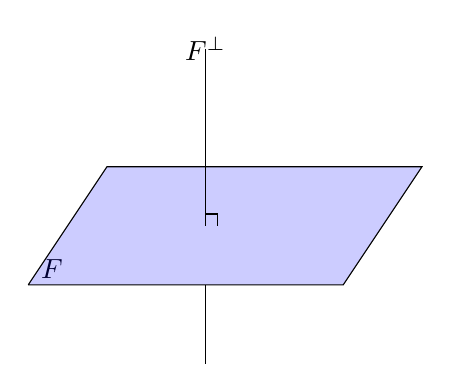
\begin{tikzpicture}
\draw (0.3,0.2) node{$F$};
\filldraw[draw=black,fill=blue, fill opacity=0.2] (0,0)--(1,1.5)--(5,1.5)--(4,0)--(0,0) ;
\draw[] (2.25,0.75)--(2.25,3)node{$F^{\perp}$} ;
\draw[] (2.25,0)--(2.25,-1) ;
\draw[] (2.25,0.9)--(2.4,0.9)--(2.4,0.75) ;		                    
\end{tikzpicture}

\end{Definition}
\begin{Proposition}
\begin{enumerate}
\item $F^{\perp}$ est un sous-espace vectoriel de $E$.
\item $F$ et $F^{\perp}$ sont en somme directe.
 \item Si $F\subset G$, alors $G^{\perp}\subset F^{\perp}.$ 
\end{enumerate}
\end{Proposition}
\begin{Demonstration}
\begin{enumerate}
\item 
\begin{itemize}
\item \textit{Non vide} : $\vect{0}\in F^{\perp}$ car  $\forall \vect{y}\in F \quad \PS{\vect{0}}{\vect{y}}=0$.
\item  \textit{Stabilité} : Soit $\vect{x},\vect{y}\in F^{\perp}$ et$\lambda,\mu\in\R$.
$$\forall \vect{z}\in F:  \quad \PS{\lambda\vect{x}+\mu \vect{y}}{\vect{z}}=\lambda\overbrace{\PS{\vect{x}}{\vect{z}}}^{=0\text{ car }\vect{x}\in F^{\perp}}+\mu\overbrace{\PS{ \vect{y}}{\vect{z}}}^{=0\text{ car }\vect{y}\in F^{\perp}}=0.$$
\end{itemize}
$F^{\perp}$ est bien un sous-espace vectoriel de $E$.
\item  
Soit $\vect{x}\in F\cap F^{\perp}$.  Donc $\PS{\overbrace{\vect{x}}^{\in F}}{\overbrace{\vect{x}}^{\in F^{\perp}}}=0$. Comme le produit scalaire est définie,  $\vect{x}=\vect{0}$.\\
$F$ et $F^{\perp}$ sont en somme directe.
\item Soit $\vect{x}\in G^{\perp}$. Soit $\vect{y}\in F$. Comme $F\subset G$, on a  $\PS{\vect{x}}{\vect{y}}=0$ puisque $\vect{x}\in G^{\perp}$. \\
On a bien $\vect{x}\in G^{\perp}$.
\end{enumerate}
\end{Demonstration}
\begin{Exemple}
On a $\{\vect{0_E}\}^{\perp}=E$ et $E^{\perp}=\{\vect{0_E}\}$ car le seul vecteur de $E$ orthogonal à tout vecteur est le vecteur nul. 
\end{Exemple}
\begin{Proposition}
$\vect{x}\in F^{\perp}$ si et seulement si $\vect{x}$ est orthogonal aux vecteurs d'une base quelconque de $F$. 
\end{Proposition}

\begin{Proposition}[Supplémentaire orthogonal d'un sous espace vectoriel de dimension finie]
Soit $F$ un espace vectoriel de dimension finie de $E$. On a :
$$E=F\oplus F^{\perp}.$$
En particulier, si $E$ est aussi de dimension finie : $\dim F^{\perp}+\dim F=\dim E$.\\
\begin{center}
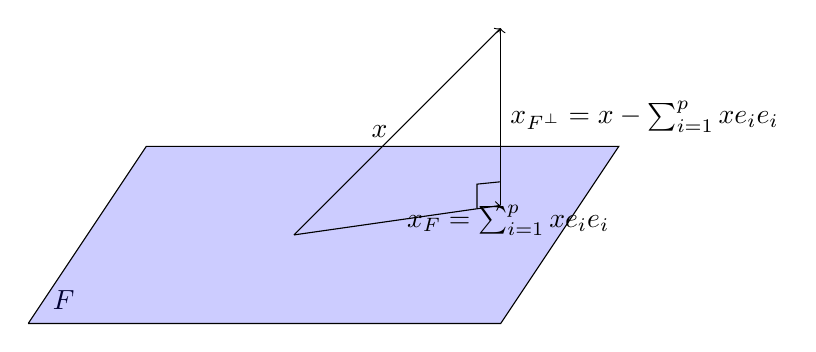
\begin{tikzpicture}[scale=1.5]
\draw (0.3,0.2) node{$F$};
\filldraw[draw=black,fill=blue, fill opacity=0.2] (0,0)--(1,1.5)--(5,1.5)--(4,0)--(0,0) ;
\draw[->] (2.25,0.75)--(4,2.5)node[pos=0.5,left]{$\vect{x}$} ;
\draw[->] (2.25,0.75)--(4,1)node[pos=0.5,above,right]{$\vect{x_F}=\sum_{i=1}^p \PS{\vect{x}}{\vect{e_i}} \vect{e_i}$} ;
\draw[->] (4,1)--(4,2.5)node[pos=0.5,right]{$\vect{x_{F^{\perp}}}=\vect{x}-\sum_{i=1}^p \PS{\vect{x}}{\vect{e_i}} \vect{e_i}$} ;
\draw[] (4,1.2)--(3.8,1.18)--(3.8,0.98) ;		                    
\end{tikzpicture}
\end{center}
\end{Proposition}
\begin{Demonstration}
Soit $(\vect{e_1},\dots,\vect{e_p})$ une base orthonormale de $F$. Soit $\vect{x}\in E$.
\begin{itemize}
\item  \textit{Analyse} : on suppose qu'il existe $\vect{x_F}=\sum_{i=1}^p x_i \vect{e_i}\in F$ et $\vect{x_{F^{\perp}}}\in F^{\perp}$ tel que :
$$\vect{x} = \sum_{i=1}^p x_i \vect{e_i} + \vect{x_{F^{\perp}}}.$$
Pour tout $k\Intf{1}{p}$, on a :
$$\PS{\vect{x}}{\vect{e_k}} = \PS{\sum_{i=1}^p x_i \vect{e_i} + \vect{x_{F^{\perp}}}}{\vect{e_k}}=\sum_{i=1}^p x_i\PS{ \vect{e_i}}{\vect{e_k}} + \PS{\vect{x_{F^{\perp}}}}{\vect{e_k}}=x_k.$$
Finalement  $\vect{x_F}=\sum_{i=1}^p \PS{\vect{x}}{\vect{e_i}} \vect{e_i}$ et $\vect{x_{F^{\perp}}}=\vect{x}-\sum_{i=1}^p \PS{\vect{x}}{\vect{e_i}} \vect{e_i}$.
\item  \textit{Synthèse} : on peut écrire 
$$\vect{x} =\overbrace{\sum_{i=1}^p \PS{\vect{x}}{\vect{e_i}} \vect{e_i}}^{\in F}+ \left(\vect{x}-\sum_{i=1}^p \PS{\vect{x}}{\vect{e_i}} \vect{e_i}\right).$$
Comme
$$\forall  j\Intf{1}{p}:\PS{\vect{x}-\sum_{i=1}^p \PS{\vect{x}}{\vect{e_i}} \vect{e_i}}{\vect{e_j}} =\PS{\vect{x}}{\vect{e_j}} -\sum_{i=1}^p \PS{\vect{x}}{\vect{e_i}}\PS{ \vect{e_i}}{\vect{e_j}}\overbrace{=}^{(\vect{e_1},\dots,\vect{e_p}) \text{ BON} }0. $$ 
$\vect{x}-\sum_{i=1}^p \PS{\vect{x}}{\vect{e_i}} \vect{e_i}$ est orthogonal à tous les vecteurs d'une base de $F^{\perp}$, donc appartient à  $F^{\perp}$.
\end{itemize}

\end{Demonstration}
\begin{Corollaire}[Inégalité de Bessel]
Soit $(\vect{e_1},\dots,\vect{e_p})$ une base orthonormale de $F$. Soit $\vect{x}\in E$.
Alors, on a :
$$\sum_{i=1}^p \PS{\vect{x}}{\vect{e_i}}^2\leq \norme{\vect{x}}^2$$
avec égalité si et seulement si $\vect{x} \in F$.
\end{Corollaire}
\begin{Demonstration}
On a :
$$\begin{aligned}
\norme{\vect{x}}^2 &=  \norme{\overbrace{\sum_{i=1}^p \PS{\vect{x}}{\vect{e_i}} \vect{e_i}}^{\in F} +\overbrace{(\vect{x}-\sum_{i=1}^p \PS{\vect{x}}{\vect{e_i}} \vect{e_i})}^{\in F^{\perp} }}^2\\
\norme{\vect{x}}^2 &\overbrace{=}^{\text{Th Pythagore}}\norme{\sum_{i=1}^p \PS{\vect{x}}{\vect{e_i}} \vect{e_i}}^2 +\norme{\vect{x}-\sum_{i=1}^p \PS{\vect{x}}{\vect{e_i}} \vect{e_i}}^2\\
\norme{\vect{x}}^2 &\overbrace{=}^{(\vect{e_1},\dots,\vect{e_p}) \text{ BON} }\sum_{i=1}^p \PS{\vect{x}}{\vect{e_i}}^2+\norme{\vect{x}-\sum_{i=1}^p \PS{\vect{x}}{\vect{e_i}} \vect{e_i}}^2\\
\norme{\vect{x}}^2 &\geq \sum_{i=1}^p \PS{\vect{x}}{\vect{e_i}}^2
\end{aligned}$$
avec égalité si et seulement si $\vect{x} \in F$.
\end{Demonstration}


%TODO rajouter l'exemple Sn et An sonst supplémentaires orthogonaux dans Mn

\subsection{Projection orthogonal et distance}
\begin{Definition}[Projecteur orthogonal]
Soit $F$ un espace vectoriel de dimension finie de $E$.\\
On appelle \defi{projection orthogonale} sur $F$ la projection, notée $p_F$, sur $F$ parallèlement à $F^{\perp}$.\\
Autrement dit, $$p_F(\vect{x})=p_F(\vect{x_F}+\vect{x_{F^{\perp}}})=\vect{x_F}=\sum_{i=1}^{n}\PS{\vect{x}}{\vect{e_i}} \vect{e_i},$$
avec $(\vect{e_1},\dots,\vect{e_p})$ une base orthonormale de $F$. 
\begin{center}
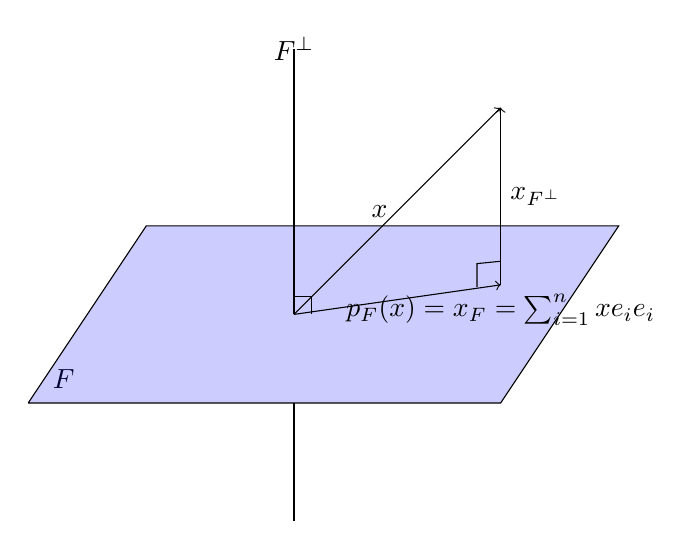
\begin{tikzpicture}[scale=1.5]
\draw (0.3,0.2) node{$F$};
\filldraw[draw=black,fill=blue, fill opacity=0.2] (0,0)--(1,1.5)--(5,1.5)--(4,0)--(0,0) ;
\draw[->] (2.25,0.75)--(4,2.5)node[pos=0.5,left]{$\vect{x}$} ;
\draw[->] (2.25,0.75)--(4,1)node[below]{$p_F(\vect{x})=\vect{x_F}=\sum_{i=1}^{n}\PS{\vect{x}}{\vect{e_i}} \vect{e_i}$} ;
\draw[->] (4,1)--(4,2.5)node[pos=0.5,right]{$\vect{x_{F^{\perp}}}$} ;
\draw[] (4,1.2)--(3.8,1.18)--(3.8,0.98) ;		                    
\draw[] (2.25,0.75)--(2.25,3)node{$F^{\perp}$} ;
\draw[] (2.25,0)--(2.25,-1) ;
\draw[] (2.25,0.9)--(2.4,0.9)--(2.4,0.75) ;		                    
\end{tikzpicture}
\end{center}
\end{Definition}

\begin{Theoreme}[Distance à un sous-espace de dimension fini]
Soit $F$ un sous-espace vectoriel de $E$ de dimension finie. Soit $\vect{x} \in E$.\\
$$\forall \vect{y} \in F, \norme{\vect{x} -\vect{y}} \geq  \norme{\vect{x} - p_F(\vect{x})}$$
 avec égalité si et seulement si $\vect{y} = p_F(\vect{x})$.
\begin{center}
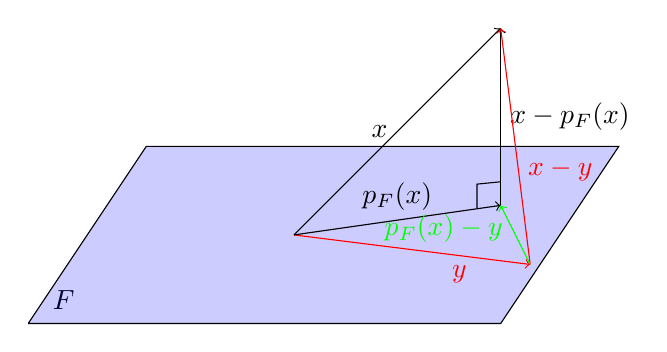
\begin{tikzpicture}[scale=1.5]
\draw (0.3,0.2) node{$F$};
\filldraw[draw=black,fill=blue, fill opacity=0.2] (0,0)--(1,1.5)--(5,1.5)--(4,0)--(0,0) ;
\draw[draw=red,->] (2.25,0.75)--(4.25,0.5)node[pos=0.7,below,red]{$\vect{y}$} ;
\draw[->] (2.25,0.75)--(4,2.5)node[pos=0.5,left]{$\vect{x}$} ;
\draw[->] (2.25,0.75)--(4,1)node[pos=0.5,above]{$p_F(\vect{x})$} ;
\draw[->] (4,1)--(4,2.5)node[pos=0.5,right]{$\vect{x} - p_F(\vect{x})$} ;
\draw[draw=red,->] (4.25,0.5)--(4,2.5)node[pos=0.4,right,red]{$\vect{x} - \vect{y}$} ;
\draw[draw=green,->] (4.25,0.5)--(4,1)node[pos=0.6,left,green]{$p_F(\vect{x})- \vect{y}$} ;
\draw[] (4,1.2)--(3.8,1.18)--(3.8,0.98) ;		                    
\end{tikzpicture}
\end{center} 
\end{Theoreme}

\begin{Demonstration}
Soit $\vect{x} \in E$ et $\vect{y} \in F$. D'après le théorème de Pythagore, on a
$$\begin{aligned}
\norme{\vect{x} - \vect{y}}&=\norme{ \overbrace{(\vect{x}- p_F(\vect{x}))}^{\in F^{\perp} }-\overbrace{(\vect{y}- p_F(\vect{x}))}^{\in F }}\overbrace{=}^{\text{Th Pythagore}} \norme{\vect{x}- p_F(\vect{x})  } +\norme{ \vect{y}- p_F(\vect{x}) }\\
\\
\norme{\vect{x} - \vect{y}}&\geq \norme{\vect{x}- p_F(\vect{x})  }
\end{aligned}$$
avec égalité si et seulement si $\vect{y} = p_F(\vect{x})$.
\end{Demonstration}
\begin{DefinitionProposition}[Distance à un sous-espace de dimension fini]
Soit $F$ un sous-espace vectoriel de $E$ de dimension finie. Soit $\vect{x} \in E$.\\
La  \defi{distance de $\vect{x}$ à $F$} est :
$$d(\vect{x},F)=\inf_{\vect{y}\in F} \norme{\vect{x} - \vect{y}} = \norme{\vect{x} - p_F(\vect{x})} .$$
\end{DefinitionProposition}
\begin{Demonstration}
C'est une conséquence directe d'un théorème précédent qui affirme que le vecteur appartenant à $F$ "le plus proche" de $\vect{x}$ est le projeté orthogonal sur $F$ de $\vect{x}$.
\end{Demonstration}
\begin{Exemple}
Soit $E=\mathbb R^2$ muni de son produit scalaire canonique et de la base canonique $\mathcal B=(\vect{e}_1,\vect{e}_2)$. On considère $F$ le sous-espace vectoriel défini par l'équation 
$$\left\{
\begin{array}{rcl}
x_1+x_2&=&0
\end{array}
\right.
$$
Déterminer la matrice dans $\mathcal B$ de la projection orthogonale $p_F$ sur $F$ puis déterminer la distance de $\vect{x}$ à $F$.
\begin{enumerate}
\item \textit{Déterminer une base orthonormale de $F$}. On commence par trouver une base de $F$. $(\vect{e}_1-\vect{e}_2)$ est une base de $F$. Cet unique vecteur constitue  une famille orthogonal, il suffit de le normaliser. Comme $\norme{\vect{e}_1-\vect{e}_2}=\sqrt{2}$, on pose $\vect{u}_1=\frac{1}{\sqrt 2} (\vect{e}_1+\vect{e}_2)$.
\item \textit{Déterminer la matrice dans $\mathcal B$ de la projection orthogonale $p_F$ sur $F$.} On calcul $p_F(\vect{e}_1)$ et $p_F(\vect{e}_2)$ par la formule $p_F(\vect{e}_i)=\PS{\vect{e}_i}{\vect{u}_1}\vect{u}_1$. On obtient :
$$[p_F]_{\mathcal{B}}=\frac{1}{2}\begin{pmatrix}
1 & -1\\
-1 & 1
\end{pmatrix}
$$
\item \textit{Déterminer la distance de $\vect{x}=(x_1,x_2)$ à $F$.} On a  $[p_F(\vect{x})]_{\mathcal{B}} = [p_F]_{\mathcal{B}}\times \begin{pmatrix}
x_1\\
x_2
\end{pmatrix}= \begin{pmatrix}
\frac{x_1 -x_2}{2} \\
\frac{-x_1 +x2 }{2}
\end{pmatrix}$. D'où $p_F(\vect{x})=(\frac{x_1 -x_2}{2},
\frac{-x_1 +x2 }{2})$. Puis $\vect{x} - p_F(\vect{x})= (\frac{x_1 +x_2}{2},\frac{x_1 +x_2}{2})$. Soit $||\vect{x} - p_F(\vect{x})||=\frac{1}{\sqrt{2}}(x1+x2)$ 
\end{enumerate}

\end{Exemple}

\section{Forme linéaire sur un espace Euclidien}
On considère un un espace euclidien réel $(E,\PS{.}{.})$.
\subsection{Représentations des formes linéaires}

\begin{Proposition}
Pour toute forme linéaire $\phi : E \to \R$, il existe un unique vecteur $\vect{u} \in E$ tel que :
$$ \forall \vect{x} \in E:\quad  \phi(\vect{x}) =\PS{ \vect{u}}{ \vect{x}} .$$
En d'autres termes, l'application $\Fonction{}{E}{E^*}{\vect{u}}{\vect{x} \mapsto \PS{ \vect{u}}{ \vect{x}}} $
est un isomorphisme.
\end{Proposition}
\begin{Demonstration}
 Soit $(\vect{e_1},\dots,\vect{e_n})$ une base orthonormale de $E$. 
Soit $\vect{x}=\sum_{i=1}^n x_i \vect{e_i}  \in E$. 
 On a :
$$ \phi(\vect{x})=\sum_{i=1}^n x_i \phi(\vect{e_i})\overbrace{=}^{(\vect{e_1},\dots,\vect{e_n})\text{ BON}}\PS{\sum_{i=1}^n \phi(\vect{e_i})\vect{e_i} }{\vect{x}}=\PS{\vect{u} }{\vect{x}},$$ 
avec $ \vect{u}=\sum_{i=1}^n \phi(\vect{e_i})\vect{e_i}$.
\end{Demonstration}


\subsection{Représentations des hyperplans}
\begin{Definition}[Vecteur normal]
Soit $H$ un hyperplan d'un espace euclidien $ E$. On appelle \defi{vecteur normal à $ H$} tout vecteur non nul orthogonal à $ H$.
\end{Definition}


\begin{Proposition}[Équation d'un hyperplan]
 Soit $ E$ un espace euclidien ayant pour base orthonormal $(\vect{e_1},\dots,\vect{e_n})$.
Soit $H$ un hyperplan de $E$. \\
Si $\vect{u}=\sum_{i=1}^n u_i \vect{e_i}$ est un vecteur normal à $H$,\\
Alors 
$$H=\left\{\vect{x}=\sum_{i=1}^n x_i \vect{e_i} \in E:   \sum_{i=1}^n u_i x_i=0 \right\}.$$
Réciproquement si 
$$H=\left\{\vect{x}=\sum_{i=1}^n x_i \vect{e_i} \in E:   \sum_{i=1}^n u_i x_i=0 \right\}$$
Alors  $\vect{u}=\sum_{i=1}^n u_i \vect{e_i}$ est un vecteur normal à $H$.\\
En d'autres termes, il existe  $\vect{u}\in E$ non nul tel que  :
$$H=\left\{\vect{x}\in E:   \PS{\vect{u}}{\vect{x}}=0 \right\}.$$
Ou bien encore, il existe $\phi \in E^*$ non nul tel que :
$$H=\ker \phi.$$ 
\end{Proposition}


%TODO APPLICATION APPROXIMATION SERIE DE FOURRIER

\end{document}
